\documentclass{aamas2010}

%\usepackage{times}
\usepackage{latexsym}
\usepackage{amsfonts,amsmath,amssymb}
\usepackage{graphicx}
\usepackage{algorithmic}
\usepackage{subfigure}



\newtheorem{Theorem}{Theorem}
\newtheorem{Lemma}{Lemma}
\newtheorem{Example}{Example}
\newtheorem{Corollary}{Corollary}
\newtheorem{Definition}{Definition}
\newtheorem{assume}{Assumption}
\newtheorem{Proposition}{Proposition}
\newtheorem{Hypothesis}{Hypothesis}


\special{papersize=8.5in,11in}

\pdfpagewidth=8.5truein
\pdfpageheight=11truein

\begin{document}

\AuthorsForCitationInfo{Anonymous}

\TitleForCitationInfo{Cultivating Desired Behaviour: Policy Teaching Via Environment-Dynamics
 Tweaks}


\title{Cultivating Desired Behaviour:\\ Policy Teaching Via Environment-Dynamics
 Tweaks}


% AUTHORS

\author{Tracking Number: 398}


\maketitle

\begin{abstract}

In this paper we study, for the first time explicitly, the
implications of allowing an interested party (i.e. a teacher) the
ability to modify the underlying \emph{dynamics} of the environment,
in order to encourage an agent to learn to follow a specific
policy. We introduce a cost function which can be used by the
interested party to balance the modifications it makes to the
underlying environment dynamics, with the learner's performance
compared to some ideal, desired, policy. We formulate the interested
party's problem of determining optimal environment changes as a
planning and control problem, and empirically validate the
effectiveness of our model.


\end{abstract}
\category{I.2.6}{Artificial Intelligence}{Learning}
\category{I.2.8}{Artificial Intelligence}{Problem Solving, Control Methods, and 
Search}[Control theory]
\category{I.2.11}{Artificial Intelligence}{Distributed Artificial Intelligence}[
Multiagent systems]
\terms{Algorithms}
\keywords{Teacher-learner, control theory, Kullback-Leibler Rate}



\section{Introduction}
%\nocite{fleming_hernandez-hernandez_CDC_97}
%\nocite{todorov_2009_framework_sup}
%\nocite{todorov_2009_framework}
%\nocite{ng_russell_2000}
%\nocite{zhang_parkes_2009_ed}
%\nocite{dufton_larson_2009}

There are three general teaching techniques applied by people:
teaching by demonstration, teaching by providing incentives, and
teaching by modifying the underlying environment dynamics.  While the
first two have been successfully mapped into intelligent agent models,
to the best of our knowledge, the third one has yet to be
instantiated.

Teaching by {\em demonstration} has a teacher provide example
state-to-action mappings in order to show the learner what a good
policy would be.  This approach has found great success in
robotics~\cite{argal_etal_2009}. However, most of these works assume
that the learner actually wishes to learn the task, as well as a
certain benevolence on behalf of the teacher with respect to the
learned task.

On the other hand, much of the work involving teaching by using {\em
  incentives} has no need to assume that the teacher's and learner's
initial interests coincide.  In particular, research in this area has
looked at ways in which a teacher could encourage or convince a
learner to follow some desired policy by providing rewards or
punishments.  Recently, Zhang \emph{et al} introduced a general
framework they call \emph{environment
  design}~\cite{Zhang09:General}. In environment design an interested
party attempts to influence the behaviour of an agent by making
limited changes to the agent's environment. Although, in general, this
may include environment dynamics modification, Zhang \emph{et al} have
concentrated on teaching by incentive. In particular, Zhang \emph{et
  al} have allowed their interested party to modify the cost function
of an agent in a linear programming example~\cite{Zhang09:General}, or
to modify the rewards of an agent acting in an environment modelled as
a Markov Decision Problem
(MDP)~\cite{zhang_parkes_2008,Zhang09:Policy}. However, these {\em
  incentive} based approaches in their current form are not
sufficiently flexible. In fact, as one of our experimental domains
demonstrates (see Section~\ref{sec: experiments}), there exist
environments where certain behaviours can not be enforced by the
method of Zhang \emph{et al}.

In this paper we explicitly focus on the implications of allowing the
interested party (teacher, in our model) to modify the \emph{dynamics}
of the environment, while leaving the reward function of the agent
alone. We term this process of teaching {\em behaviour
  cultivation}. In more detail, we concentrate on environments
modelled by the learner as an MDP, and allow the teacher to
\emph{tweak} (\emph{i.e.} make small changes to) the environment
dynamics and record the outcome within the MDP model.  The teacher's
goal is, therefore, to determine the form and the degree of tweaking
necessary to enforce a specified behaviour upon the learner.


While our model may be cast as an example of environment design, we
note that our instantiation differs significantly from the particular
cases studied by Zhang \emph{et al}, and therefore creates a separate
line of study. In fact, representing the teacher's task as a control
problem is far more reminiscent of the work by Banerjee and
Peng~\cite{banerjee_peng_2005}. In~\cite{banerjee_peng_2005} an
additional assumption is made about the size of the learner's memory
and the fact that the teacher-learner interaction is based on a
repeated normal form game. This enabled Banerjee and Peng to enumerate
all possible memory configurations and use them as a system state
space, casting the interaction between the teacher and its opponent as
a planning and control problem termed Adversary MDP. Solving this
problem allows the teacher to force its opponent to follow a strategy
which is most beneficial from the teacher's utility point of
view. However, their method provides no formal way of achieving a
prespecifed behaviour of the learner, as well as being limited to a
finite set of memory configurations, hardly a feasible situation even
for a learning algorithm in a simple repeated normal form game.

We believe that the power of our learning model is best illustrated by
the following real-world scenario. A parent wishes to teach a child to
ride a bicycle. The parent may {\em demonstrate} by riding the
bicycle. However, in practice, this does not yield good results when
the child attempts to repeat the task. It is also possible to promise
an {\em incentive}, be that a candy or a trip to the
park. Unfortunately, although increasing the child's efforts, this
does not facilitate the learning process. The most practical thing to
do, in this case, is to {\em modify the dynamics} -- add safety wheels
to the bicycle. Gradually raising the safety wheels constitutes {\em
  behaviour cultivation}. It ultimately allows the child to accustom
to the complete range of motion possibilities and, eventually, ride an
unabridged bicycle version. Another good example, this time with
multiple agents, would be the task a coach faces when introducing a
new player into his football team. The new player has to be accustomed
to this team's play-book (a set of attack and defence plans), but also
the rest of team has to be trained to incorporate the unique set of
skills brought in by the new player. Here too, neither {\em
  demonstration} nor {\em incentives} work very well. Rather, the
coach has to create a sequence of drills where the new player's skills
and the old play-book will be gradually integrated. These drills do
not possess the complete complexity and dynamics of the real football
game, instead they gradually approximate the real game dynamics, and
constitute {\em behaviour cultivation}. Ultimately, a full scale
football match is played, where the coach no longer influences the
game rules or dynamics.

The contributions of this work are three-fold:
\begin{itemize}
\item We introduce a model whereby a teacher can modify or tweak
  environment dynamics so as to cultivate some desired behaviour in a
  learning agent. This is the first time the {\em behaviour
    cultivation} teaching method is considered explicitly.
\item We introduce a cost function for the teacher that naturally
  incorporates and balances the teacher's effort and the deviation of
  the learner's performance from an ideal reference, that which the
  teacher is interested in. Such balance is an important feature for
  multi-aspect optimisation, and otherwise would have necessitated a
  separate treatment.
\item We instantiate our model with a particular learning agent, and
  then show, empirically, that our model is effective. Our {\em
    behaviour cultivation} method was able both to speed up a normal
  learning process and solve teaching tasks which are hard or
  impossible for other methods.
\end{itemize}

%To achieve this goal, we first introduce a way to measure the
%divergence between the realised and the passive (when no modification
%is applied by the teacher) environment developments in a Markovian
%system. This measure naturally incorporates and balances the teacher's
%effort and the deviation of the learner's performance from an ideal
%reference, that which the teacher is interested in. It also allows us
%to formulate the teacher's problem as a planning and control problem,
%and solve it using classical analytical and numerical tools.

The rest of this paper is organised in the following manner. In
Section~\ref{sec: GeneralModel} we present our general model for
\emph{behaviour cultivation}, and describe the cost function, which is
based on the Kullback-Leibler Rate, that we use.  In Section~\ref{sec:
  TOP-PI} we instantiate our general model with a particular type of
learning agent, one that uses a Policy Iteration algorithm to
determine which policy it will follow. Using this instantiation, we
show, in Section~\ref{sec: experiments}, that our model is effective,
before concluding in Section~\ref{sec: future work} with a discussion
of future research directions.


%In what follows we will formally define {\em behaviour cultivation}
%process that can be parameterised by the learning algorithm we wish to
%teach(Section~\ref{sec: GeneralModel}).
%%teaching by dynamics
%%modification 
%%given a learning algorithm we wish to teach
%%. 
%We will also provide a specialised
%version of the formalism for a specific MDP solution technique --
%Policy Iteration (PI) algorithm (Section~\ref{sec: TOP-PI}). $\{\{$
%Our experiments in Section~\ref{sec: experiments} will compare the
%performance of PI with and without dynamics modification. $\}\}$. We
%will then conclude in Section~\ref{sec: future work} with a discussion
%of further development teaching by dynamics modification.




%%%%%%%%%%%%%%%%%%%%%%%%%%%%%%
\section{Interaction Model}\label{sec: GeneralModel}
%%%%%%%%%%%%%%%%%%%%%%%%%%%%%%

In this section we provide a high level description of the problem and
general framework.  In the next section we provide a particular
instantiation of our framework.

Our framework consists of a stochastic environment and two agents, a
\emph{learner} and a \emph{teacher}.  The learner acts within the
environment, taking actions and receiving feedback in the form of
rewards, which depend on the action taken and the current state of the
environment in which the agent finds itself.  We assume that the
learner is rational and thus attempts to find a \emph{policy} which
describes what action to take in each environment state, so as to
maximises its expected reward.  The teacher, on the other hand, does
not act \emph{in} the environment, but rather acts \emph{on} the
environment.  In particular, the teacher has some desired
\emph{reference policy}, $\pi^*$, that it wishes the learner to
follow, but is unable to force the agent to take any particular
action.  Instead, it  it is able to modify the environment's
\emph{dynamics} in order to cultivate the desired behaviour in the learner.  That is, the teacher's actions are able to influence the way
the environment state changes in response to the learner's actions,
and thus influence the policy of the learner. Dynamics modifications, or \emph{tweaks}, 
come at a cost, however, and thus the goal of the teacher is to
minimise the modifications it must make to the environment dynamics
while at the same time ensuring that the policy followed by the
learner is close enough to the desired reference policy.

We represent  the problem with the tuple  $\langle S, A, c,\gamma, U,T\rangle$ where:
\begin{itemize}
\item $S$ is the set of states, 
\item $A$ is the set of actions available to the learner,
\item  $c:S\times A\times S\rightarrow\mathbf{R}$ is the reward (or
  cost) function of the learner. $c(s',a,s)$ is the reward received by
  the learner if it has applied action $a\in A$ and the environment
  moved from state $s\in S$ to state $s'\in S$,
\item $\gamma \in (0,1)$ is a discount factor,   

\item $U$ is the set of actions (modifications to the environment)
  that the teacher can apply where $u_t\in U$ is the modification or tweak made
  at time $t$,

\item $T:S\times A\times U\rightarrow\Delta(S)$ describes the
  environment dynamics where $T_u(s'|s,a)\equiv T(s'|s,a,u)$ is the
  probability that the state will change from $s$ to $s'$ if the
  learner has applied action $a\in A$ and the teacher chose
  environment modification $u\in U$.

We assume that there exists a null modification $u^0\in U$, so that
$T^0=T_{u^0}$  are the original dynamics of the environment before any teacher-modifications. We will use the term \emph{passive dynamics} to refer to $T^0$ to highlight the fact that it is unchanged.

\end{itemize}

We assume that the learner modifies and updates its policy by using some iterative algorithm, such 
as value or policy iteration.  In between iterations, the teacher is able to apply a tweak or 
modification to the environment dynamics, and thus, the learner faces 
 a sequence of Markov Decision Problems (MDPs)~\cite{puterman_book_94},
 given by tuples $<S,A,U,T_{u_t},R>$. We assume that the learner is unaware of the teacher's  
 actions, and thus proceeds as if the sequence of MDPs were homogeneous.
 
 
\begin{assume}\label{assume_persistence}
At every
stage the learner seeks an action policy of the form
$\pi:S\rightarrow\Delta(A)$ that would produce the highest expected
reward if $T_{u_t}$ would persist indefinitely.\footnote{This 
  assumption is explicit only if the learner actually has access to
  the environment model. For most standard reinforcement learning algorithms this
  assumption would hold implicitly.}
\end{assume}


Let $x_t$ represent all information and features that the learner uses
in determining its policy, and let
$\pi_t=\pi(x_t):S\rightarrow\Delta(A)$ be the policy that corresponds
to that state.  Additionally, let $\pi^*$ be the ideal policy that the
teacher desires the learner to follow.  At time $t$, the teacher
incurs a cost, $\mathrm{Cost}(\pi_t,u_t)$, which combines the
difference between the actual policy being followed by the learner,
$\pi_t$, and the desired policy of the teacher, $\pi^*$, with the
amount of environmental modifications the learner has had to make in
order to maintain the current dynamics, $T_{u_t}$, compared to the
initial environment dynamics, $T^0$. If we let $x_t=F(x_{t-1},u_t)$
denote one step of the learner's policy-determination algorithm and
assume that $x_0$, the original state of the learner,  is known, then it is possible to formulate the overall optimisation problem faced by the teacher.
In particular, it is:
\begin{eqnarray*}
&\min\limits_{u_t}\sum\limits_{t=1}^{t_{max}}Cost(\pi_t,u_t)\\
&s.t.\\
&\pi_t=\pi(x_t)\\
&x_t=F(x_{t-1},u_t).
\end{eqnarray*}



%Now, denote $x_t$ the internal state of the learner's policy
%computation at iteration $t$, and let
%$\pi_t=\pi(x_t):S\rightarrow\Delta(A)$ be the policy that corresponds
%to that computation state. Also, denote $\pi^*$ the ideal reference
%action policy of the learner. Then at time $t$ the teacher incurs cost
%$Cost(\pi_t,u_t)$ that combines the distance between $\pi_t$ and
%$\pi^*$ and between $T_{u_t}$ and $T^0$. The overall optimisation
%problem for the teacher is as follows, where $x_t=F(x_{t-1},u_t)$
%denotes one step of the learner's computation algorithm and $x_0$ is
%known:
%\begin{eqnarray*}
%&\min\limits_{u_t}\sum\limits_{t=1}^{t_{max}}Cost(\pi_t,u_t)\\
%&s.t.\\
%&\pi_t=\pi(x_t)\\
%&x_t=F(x_{t-1},u_t)
%\end{eqnarray*}

This formulation of the teacher's optimization function is fully generic. It does not explicitly specify 
the learner's algorithm beyond assuming that it is iterative. This formalism thus captures both policy 
and value iteration algorithms, both with given and learned environment models.
It can also
 capture the case where the learner
is capable of transfer learning~\cite{ taylor_stone_2009}. In this scenario the learner's state $x_t$
will include structural knowledge gathered thus far from the
interaction with the environment. 

Our teacher-learner interaction framework, as described, is also generic with respect to the 
instantiation of the teacher's cost function, $Cost(\pi_t,u_t)$. We argue that suitable cost functions 
for this problem should incorporate information as to what environmental modifications the teacher 
has performed (\emph{i.e.} the actions taken by the teacher), along with information about how 
similar the policy of the learner is to the desired policy of the teacher (\emph{i.e.} how far the 
teacher is from its goal). While any function which combines these features in a meaningful way 
would work, in this paper we adopt a specific cost function derived from the \emph{Kullback-Leibler 
Divergence Rate}.    We describe our proposed cost function in more detail in the next section.



\subsection{Teacher's Cost Computation}\label{sec:KLCost}

In this section we describe our cost function, based on the 
 Kullback-Leibler Divergence Rate (KL Rate).  We first provide some background material on 
 Kullback-Leibler Divergence (KL Divergence) and KLR. We then describe how our cost function is 
 defined, 
 and provide an argument as to why it is appropriate for our setting.


\begin{Definition}
Let $p$ and $q$ be probability distributions over some discrete random variable. Then the Kullback-Leibler (KL) Divergence of $q$ from $p$  is
\[
D^{KL}(p||q)=\sum_i p(i)\log \frac{p(i)}{q(i)}.
\]
\end{Definition}

\noindent Informally, KL Divergence measures the difference between two probability distributions.
KL Rate is an extension of KL Divergence to Markov processes.
\begin{Definition}
Let $\{X^1_t\}$ and $\{X^2_t\}$ be Markov Processes.  The Kullback-Leibler (KL) Rate is
\[
KLR(X^1||X^2)=\lim_{n\rightarrow \infty} \frac{1}{n}DL^{KL}(P(X^1=x_n)||P(X^2=x_n)).
\]
\end{Definition}
If the processes can be described by two conditional transition matrices, $P$ and $Q$, where $P(x'|x)$ (and  respectively $Q(x'|x)$) is the probability of transitioning from state $x$ to state $x'$, then
\[
KLR(X^1||X^2)=\sum_{x} D^{KL}(P(\cdot|x)||Q(\cdot|x))p_{stat}(x)
\]
where $p_{stat}$ is the stationary distribution of $P$~\cite{rached_alajaji_campbell_2004}.


Now, returning to our problem, let $\pi_t$ be the policy of the learner at time $t$ and let $T_{u_t}$ 
be the dynamics of the environment after the teacher has applied tweak $u_t$. If $\pi_t$ was to be 
repeatedly used in the environment modified by $u_t$, this would result in a homogeneous 
Markovian process defined by the transition matrix
\[
P_t(s',a'|s,a)=T_{u_t}(s'|s,a)\pi_t(a'|s').
\]
Similarly, we can define another  Markovian process by the transition matrix
\[
P^*(s',a'|s,a)=T^0(s'|s,a)\pi^*(a'|s').
\]
This is the ideal stochastic process over state-action pairs, from the teacher's perspective. In 
particular, it is formed when the teacher's desired policy, $\pi^*$, is followed by the learner in the 
original, unmodified environment. That is, the learner executes the teacher's desired policy with no 
intervention from the teacher.

Assuming that $P_t$ and $P^*$ are irreducible with respect to $S\times A$,  we define our cost function as
\begin{eqnarray*}
Cost(u_t,\pi_t) & =& KLR(P_t||P^*) \\
                           &=& \sum_{s,a}D^{KL}_t(s,a)q_t(s,a)
\end{eqnarray*}
where
\[
D_t^{KL}(s,a)=D^{KL}(P_t(\cdot,\cdot|s,a)||P^*(\cdot,\cdot|s,a))
\]
and $q_t(s,a)$ is the  stationary distribution of $P_t$, so that
$q_t=P_tq_t$. 
Notably, the
stationary distribution can be decomposed (with a slight abuse of
notation) to be $q_t(s,a)=q_t(a|s)q_t(s)$ and then expressed by the
following equations:
%% \begin{eqnarray*}
%% q_t&=&q_t(a'|s')q_t(s')=P_tq_t\\
%% &=&\sum\limits_{s,a}T_{u_t}(s'|s,a)\pi_t(a'|s')q_t(a|s)q_t(s)\\
%% &=&\pi_t(a'|s')\sum\limits_sq_t(s)\sum\limits_aT_{u_t}(s'|s,a)q_t(a|s)\\
%% &&\{\displaystyle{substitute}\ \ q_t(\cdot|\cdot)\Leftarrow\pi_t(\cdot|\cdot)\}\\
%% &=&\pi_t(a'|s')\sum\limits_sq_t(s)\sum\limits_aT_{u_t}(s'|s,a)\pi_t(a|s)\\
%% &&\{\displaystyle{denote}\ \ \Tilde{T}_{u_t}(s'|s)=\sum\limits_aT_{u_t}(s'|s,a)\pi_t(a|s)\}\\
%% &=&\pi_t(a'|s')\sum\limits_sq_t(s)\Tilde{T}_{u_t}(s'|s)
%% \end{eqnarray*}
%% so that
\begin{eqnarray*}
q_t(s',a')&=&\pi_t(a'|s')q_t(s')\ \ \mbox{where}\\
q_t(s')&=&\sum\limits_s\Tilde{T}_{u_t}(s'|s)q_t(s) \ \ \mbox{and}\\
\Tilde{T}_{u_t}(s'|s)&=&\sum_{a}T_{u_t}(s'|s,a)\pi_t(a|s).
\end{eqnarray*}



Incorporating our KLR-based cost function, the overall generic Teacher
Optimisation Problem (TOP) is depicted in Figure~\ref{t_opt}. 

Notice
that this formulation retains complete flexibility with respect to the
specific algorithm selected by the learner to optimise its
policy. Nevertheless, to provide further intuition and demonstrate the
feasibility of the approach, in the rest of this paper we instantiate
the algorithm $F$ to be the Policy Iteration algorithm. However,
before proceeding  to this particular instantiation, we would like to
remark upon the meaning of the use of KLR and KL Divergence in our teaching problem.

%%%%%%%%%%%%%%%%%
\begin{figure}[ht]
\begin{tabular}{|c|} \hline \parbox{3.2 in} {\center 
$\arg\min\limits_{u_t}\sum\limits_{t=1}^{t_{max}}\sum\limits_{s,a}\pi_t(a|s)q_t(s)D^{KL}_t(s,a)$\\
s.t.\\
$\pi_t=\pi(x_t)$\\
$x_t=F(x_{t-1},u_t)$\\
$x_0\ \ \displaystyle{is\ \ given}$\\
$D^{KL}_t(s,a)=\sum\limits_{s',a'}T_{u_t}(s'|a,s)\pi_t(a'|s')\log\frac{T_{u_t}(s'|a,s)\pi_t(a'|s')}{T^0(s'|a,s)\pi^*(a'|s')}$\\
$q_t(s')=\sum\limits_s\Tilde{T}_{u_t}(s'|s)q_t(s)$\\
$\Tilde{T}_{u_t}(s'|s)=\sum\limits_aT_{u_t}(s'|s,a)\pi_t(a|s)$\\\ \\
}\\ \hline \end{tabular}
\caption{\label{t_opt}The complete generic TOP}
\end{figure}
%%%%%%%%%%%%%%%%%%%%%%%%%%%%%%

As we mentioned in the start of this section, KL Divergence,
$D^{KL}(P||Q)$, informally measures the difference between some
factual distribution $P$ and some desired distribution
$Q$.\footnote{Note that while KL Divergence is often called the
  \emph{distance} between two distributions, it is, in fact, not a
  true distance metric.}  As expected, $D^{KL}(P||Q)$ is minimized
exactly when $P=Q$, that is, $D^{KL}(P||P)=0$. Importantly, it
compares two distributions, rather than distribution properties, such
as the mean or variance which are commonly used. \footnote{Consider,
  for instance, the optimality criterea of MDPs: the {\em expected}
  accumulated reward. Rather than being concerned with the entire
  shape of the obtainable rewards, it only concentrates on the
  expecations, neccessitating further solution augmentation to account
  for requirements such as risk-aversion.}. In our problem, the
desired distribution is $P^*(s',a'|s,a)$ which arises if the learner
follows the teacher's desired policy with no environmental tweaks
required.  By using KLR as the cost function, we are able to assign
costs to the complete variety of possible long term deviations caused
by departing from the ideal probability of state-action pair
transition.  These deviations may arise from either the environmental
tweak made by the teacher, or by the learner following a non-desired
policy, or some combination of both, and thus our cost function
balances these appropriately.

%Originally, $KL$ divergence (and KRL) was designed to measure the cost
%of mistaken encoding. That is, if a signal had come from a
%distribution $P$, while we have used a distribution $Q$ to encode it,
%$KL(P\|Q)$ measures the extra bits we had to
%use\cite{cover_thomas_IT_book_91}. Therefore, given the signal,
%information theory seeks to recover $Q$ to minimise the extra cost. In
%our teaching domain, the signal is the sequence of state-action pairs
%engendered by the system dynamics and the learning algorithm. However,
%by changing the system dynamics we essentially change the signal true
%distribution, rather than its encoding. Hence, we represent the ideal
%policy and the passive dynamics as the encoding distribution $Q$,
%while we modulate the signal distribution $P$ to match it.






\section{TOP with Policy Iteration}\label{sec: TOP-PI}
The standard policy iteration (PI) algorithm is an iterative algorithm
that operates over an explicitly given MDP\cite{puterman_book_94}, and
it has two principal stages: policy evaluation and policy
improvement. At the the {\em policy evaluation} stage PI computes the
reward gained by applying currently considered policy. Specifically,
given the policy of the previous iteration, $\pi_{t-1}$, the value
function $V_t(s)$ for that policy is computed, where $V_t(s)$
represents the expected total discounted reward that can be achieved
if the environment starts at state $s$ and the agent follows
$\pi_{t-1}$. At the {\em policy improvement} stage the value function
of the current policy is used to guide the computation of the next
stage policy. Commonly, it is a policy $\pi_{t}$, which is optimal
policy, given the $V_t(s)$.

Since its original introduction, both stages of the algorithm have
been refined to enable partial knowledge of the domain or introduce
conservative safety features. For instance, the value function can be
estimated, rather than computed, in environment where a direct
computation is too complex or impossible due to poor modelling by the
learner. Another possible extension is introduction of safety features
into the calculations of the new policy (e.g risk aversion). Such
modifications have been extensively used, particularly in robotics,
leading to more and more advanced methods (see
e.g.~\cite{sugiyama_et_al_2009}). Hence, by making basic PI method our
study subject in this paper, we intend to impact a large cross-cut of
applications where these learning techniques are used in a
teacher-learner (or leader-follower) setup.

In more detail, we consider the standard PI algorithm, where the
environment model is completely known and the value function is
directly computed. However, for the reasons of computational
convenience, we do introduce a modification into the policy
improvement stage. Namely, the new policy is computed as a
soft-maximisation with respect to the value function. This is done to
support differentiability of the policy with respect to the
environment dynamics\footnote{Quite commonly PI is used in combination
  with a form of neural-network computation, where soft-max is a
  natural property. As a reslt our modification does not breach the
  boundaries of the acceptable practice.}.
Formally instantiating our learner's state update $F(x_t,u)$ by PI
leads to the following set of equations:\\\ \\
{\em Policy evaluation:}\\
\centerline{
  $V_t(s)=\sum\limits_{s'}T_{u_t}(s'|s,\pi_{t-1}(s))\left[
    c(s',\pi_{t-1}(s),s)+\gamma V_t(s')
    \right]$}
{\em Policy improvement:}\\
\centerline{
$\pi_t(a|s)=\frac{1}{Z_t(s)}\exp\left(\tau_t\sum\limits_{s'}T_{u_t}(s'|s,a)\left[
    c(s',a,s)+\gamma V_t(s')
    \right]\right)$}
{\em Normalisation factor:}\\ 
\centerline{
$Z_t(s)=\sum\limits_a\exp\left(\tau_t\sum\limits_{s'}T_{u_t}(s'|s,a)\left[
    c(s',a,s)+\gamma V_t(s') \right]\right)$}

The parameter
$\tau_t$ denotes a temperature scale that shifts the soft-max towards
the greedy maximum selection. Substituting the above into the standard
TOP formulation leads to a TOP-PI optimisation problem depicted in
Figure~\ref{t_opt_PI}.
\begin{figure}[th]
\begin{tabular}{|c|} \hline \parbox{3.2 in} {\center 
$\arg\min\limits_{u_t}\sum\limits_{t=1}^{t_{max}}\sum\limits_{s,a}\pi_t(a|s)q_t(s)D^{KL}_t(s,a)$\\
$s.t.$\\
$V_t(s)=\sum\limits_{s'}T_{u_t}(s'|s,\pi_{t-1}(s))\left[
c(s',\pi_{t-1}(s),s)+\gamma V_t(s')
\right]$\\
$\pi_t(a|s)=\frac{\exp\left(\tau_t\sum\limits_{s'}T_{u_t}(s'|s,a)\left[
c(s',a,s)+\gamma V_t(s')
\right]\right)}{Z_t(s)}$\\
$Z_t(s)=\sum\limits_a\exp\left(\tau_t\sum\limits_{s'}T_{u_t}(s'|s,a)\left[
c(s',a,s)+\gamma V_t(s')
\right]\right)$\\
$\pi_0\ \ \displaystyle{given}$\\
$D^{KL}_t(s,a)=\sum\limits_{s',a'}T_{u_t}(s'|a,s)\pi_t(a'|s')\log\frac{T_{u_t}(s'|a,s)\pi_t(a'|s')}{T^0(s'|a,s)\pi^*(a'|s')}$\\
$q_t(s')=\sum\limits_s\Tilde{T}_{u_t}(s'|s)q_t(s)$\\
$\Tilde{T}_{u_t}(s'|s)=\sum\limits_aT_{u_t}(s'|s,a)\pi_t(a|s)$\\\ \\
}\\ \hline \end{tabular}
\caption{\label{t_opt_PI}TOP-PI: The complete and explicit TOP for the
  PI learner}
\end{figure}

\section{Experimental Demonstration}\label{sec: experiments}
Consider a learner agent that is tasked with finding an optimal path
for supply transportation between point $S$ and $T$ on a grid. The
learner's reward is initially fixed to be $-1$ for every step it takes
plus some values $R_{ST}$ and $R_{TS}$ for reaching point T from S and
vice versa. In a uniform grid this would be a simple problem, however,
the grid simulates a terrain and cells have an associated elevation.  
As a result, any movement from one cell to another neighbouring cell
succeeds with a probability proportional to the relative elevation of 
the cells. Consider the situation depicted in Figure~\ref{exp_motion}. 

\begin{figure}[ht]
\centerline{\psfig{file=img/exp_motion.eps,width=5cm}}
\caption{\label{exp_motion}Example of a 3D terrain grid.}
\end{figure}

If the cells are of equal elevation, the movement almost always
succeeds, e.g. moving from cell $B$ to cell $C$ in
Figure~\ref{exp_motion}. If the source cell of the motion is lower
than the target cell, then the motion succeeds with low
probability. Furthermore, in this case, a non-zero probability exists
that the direction of motion will be altered. E.g. moving from $H$ to
$E$ is unlikely to succeed, and the agent may end up in $D$, $F$ or
even $G$. If the motion is directed to lower the elevation, it is most
likely will succeed, but also has certain probability to move further
than intended. E.g. moving from $B$ to $E$ is likely to succeed, but
the agent may end up in $H$ or $G$.

Finding an optimal path of motion from $S$ to $T$ and back is,
therefore, becomes non-trivial. Still, if the probabilities of
different transitions are given, the policy iteration algorithm can
easily solve the problem. However, the time it takes the algorithm to
converge to an optimal policy may vary depending on how prominent are
the features of the terrain. Therefore it would be reasonable to
assume that scaling the terrain (and modifying transition
probabilities accordingly) during the initial iterations of learning,
or shaping the landscape to ``push'' the agent in the right direction
will result in faster convergence to the optimal solution. Our
experiments are directed to verify this proposition using our TOP-PI
formalism.  We also test the efficacy of directing the agent to follow
a specific path, different to the optimal, from $S$ to $T$ using TOP-PI.

For our experimental verification we consider a $4 \times 4$ grid world where the learner can move in any cardinal direction or stay put.  Each cell has a randomly assigned elevation, shown in Figure~\ref{probalt}, that modifies the dynamics of each action as described above.  The learner has a reward of $+1$ for any actions ending in the target state and $-1$ otherwise.  This results in an optimal policy of heading toward the target state in the shortest number of steps (see Figure~\ref{prevopt}).  The learner uses policy iteration to find a policy maximising expected discounted sum of future rewards.  The teacher can arbitrarily modify the underlying dynamics of the environment

\begin{figure}[ht]
\centerline{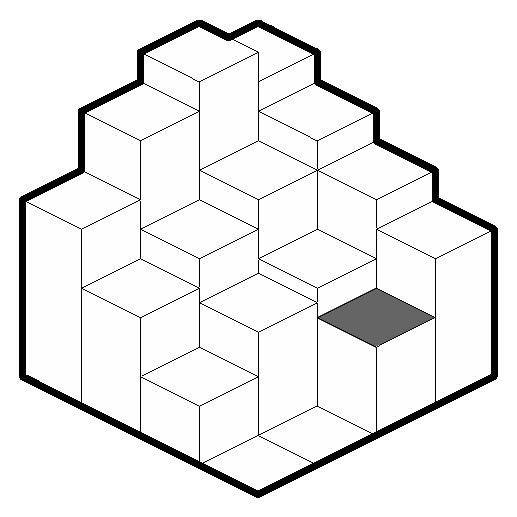
\psfig{file=img/probalt.eps,width=5cm}}
\caption{\label{probalt}The unmodified 3D terrain.}
\end{figure}

\begin{figure}[ht]
\centerline{\psfig{file=img/prevopt.eps,width=5cm}}
\caption{\label{prevopt}Original optimal policy of our test grid.  The shaded cell is the target state, with the policy action to remain put.}
\end{figure}

In our test environment, the information about the reward state can take multiple iterations of policy iteration to propagate to all other states.  This leaves the learner to make arbitrary guesses in early iterations.  By using TOP-PI, we found that the teacher was able to shape the dynamics such that the agent is ``pushed'' in the appropriate direction from the beginning.  Without the teacher modifying the dynamics, the learner required $4$ iterations of PI to find the optimal policy.  With the addition of the teacher, the modified dynamics led the learner to follow the target policy in $3$ iterations.

\begin{figure}[ht]
\centerline{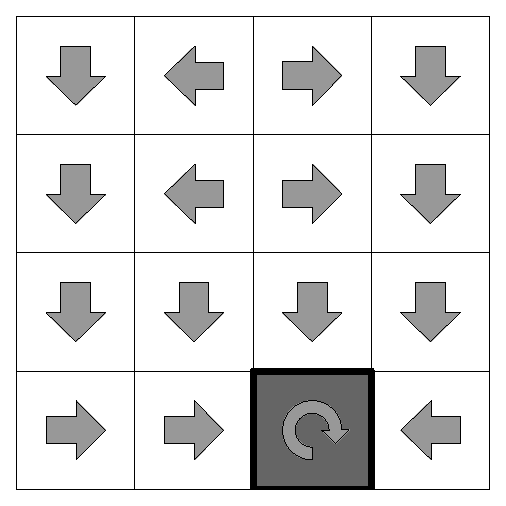
\psfig{file=img/newopt.eps,width=5cm}}
\caption{\label{newopt}A target policy that avoids centre cells.}
\end{figure}

\begin{figure}[ht]
\centerline{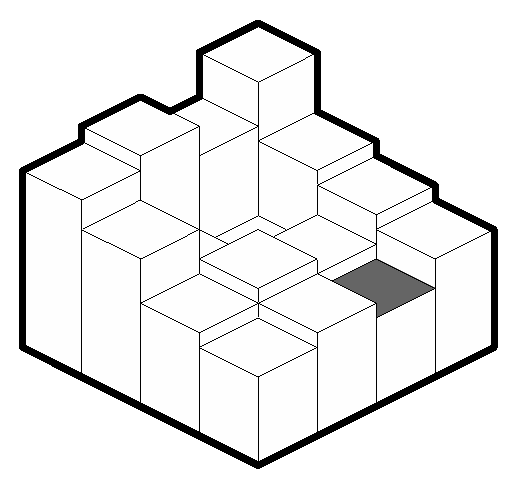
\psfig{file=img/newalt.eps,width=5cm}}
\caption{\label{newalt}An impression of the new terrain corresponding to the modified dynamics at the final iteration.}
\end{figure}

We also tested modifying the optimal policy of the MDP through tweaked dynamics.  Our test problem modified the optimal policy from a simple shortest path to the reward state to one that avoids the centre states and follows the edge states to the goal (see Figure~\ref{newopt}).  Our tests showed that this policy modification was achieved through the modifications, provided by the teacher, to the environment dynamics.   With the teacher using TOP-PI on the new target policy, the learner found this new policy using Policy Iteration in $4$ iterations.  Although in these experiments the terrain is not modified explicitly, an impression of the new terrain based on the tweaked dynamics of the final policy iteration is shown in Figure~\ref{newalt}.  In this domain with a maximum number of policy iterations for TOP-PI of $4$ the modifications to the dynamics tended to quite large, with the average change in each entry of the environmental dynamics $T$ ranging from $0.058$ in the first iteration to $0.036$ in the final iteration.

This policy modification method allows changes that are not possible with modifications to the reward function alone.  In our test on a $2 \times 2$ grid, we changed the policy as in Figure~\ref{envdopt}.  By modifying the reward function to achieve this policy the reward values must be strictly increasing along the path, otherwise it would be optimal to remain put.  This means the reward for the upper-left state must be less than the reward for the lower right (target) state, so the optimal action for lower-left would be to move right rather than up.  However, tweaking the dynamics allows such a policy modification.

\begin{figure}[ht]
\centerline{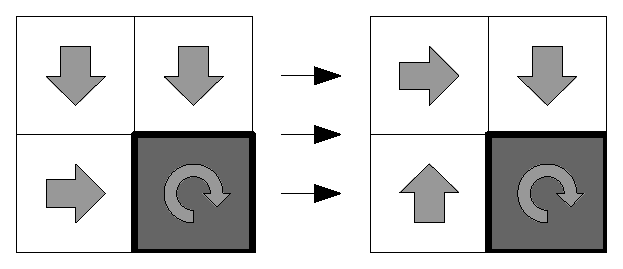
\psfig{file=img/envdopt.eps,width=5cm}}
\caption{\label{envdopt}The original optimal policy (left) and target policy (right).}
\end{figure}

Our experiments provided experimental verification of our proposed teaching method.  We verified that the method can be used both to speed up the learning process and tested this on policy iteration.  We also found that the method is able to direct the learner to a different policy by changing the dynamics of the environment.

\section{Conclusions and Future Work}\label{sec: future work}

In this paper we have introduced a novel interaction framework between
a teacher and a learner agents. Unlike previous developments in this
area, in our framework the teacher influences the learner indirectly by
modifying the environment away from some normative, passive
dynamics. We term this process {\em behaviour cultivation}.

Our approach completes the polytomy of feasible teacher-learner
interactions, forming a rigorously studied triad: by demonstration, by
incentive, and by behaviour cultivation. Although the latter two can
be unified under the umbrella of the environment
design~\cite{Zhang09:General}, with some of the ideology tracing back
to Hammond and Converse~\cite{hammond_converse_91}, the members of the
teaching triad are, in fact, distinct. Furthermore, while the
difference in their mathematical formalism can be seen as an outcome
of some representation convenience, the diversity in their
applicability argues that each of them is irrevocably necessary.

%Our approach completes the polytomy of feasible teacher-learner
%interactions, forming a rigorously studied triad: by demonstration, by
%incentive, and by behaviour cultivation. Although the ideology of the
%latter two can be unified under the umbrella of environment
%design~\cite{Zhang09:General}, which in turn can be traced back to at
%least 1991~\cite{hammond_converse_91}, the members of the teaching
%triad are, in fact, distinct. While the difference in their
%mathematical formalism can be seen as an outcome of the representation
%convenience, the diversity in their applicability argues that each of
%them is irrevocably necessary.

In particular, we have provided an experimental domain that could not
be addressed by neither {\em demonstration} (because the teacher's and
the learner's interests in the task contradict) nor currently
available {\em incentive} based methods (because incentives created a
reasoning paradox in the task), but was successfully resolved using
our {\em behaviour cultivation} teaching method. In general, as an
important part of our future work we see the classification of various
teacher-learner tasks into groups that are more suitable for a
particular teaching method.

%As an important part of our future work we see the classification of
%various teacher-learner tasks into groups that are more suitable for a
%particular teaching method. As a part of this effort, we have provided
%an experimental domain that could not be addressed by neither {\em
%  demonstration} (because the teacher's and the learner's interests in
%the task contradict) nor currently available {\em incentive} based
%methods (because incentives created a reasoning paradox in the task),
%but was successfully resolved using our {\em behaviour cultivation}
%teaching method.

Although in this paper we provide an example based on a learner
executing the policy iteration (PI) algorithm, this limitation is not
a part of our Teacher Optimisation Problem (TOP) framework. Rather it
is a particular instantiation of its principles for the PI
algorithm. We hope that the wide applicability of PI-type algorithms
will allow for a faster adoption of our {\em behaviour cultivation}
method by the multi-agent systems research community. As part of our
ongoing research we will investigate the instantiations of TOP with
other learning algorithms, particularly those capable of knowledge
transfer~\cite{taylor_stone_2009,taylor_PhD_2008}.

The cost and the effectiveness of the teaching process in TOP can be
measured simultaneously via the Kullback-Leibler divergence rate
(KLR). Specifically, by measuring the KLR between two state-action
processes engendered by the learner's action policy and the
environment dynamics set by the teacher. The detailed choice of the
two processes depends on the interpretation of this cost. One such
interpretation, as the effort it takes to sustain the teaching process
at any given time, is adopted in this paper. As a result the cost is
the KLR between the current policy-environment combination and the
combination of the reference policy with the passive dynamics.

Although ideologically this choice of the cost function is similar to
works by
Todorov~\cite{todorov_2009_framework,todorov_2009_framework_sup}, its
integration with the interaction model is different. Furthermore, we
use KL {\em rate}, rather than KL {\em divergence} used by
Todorov. This allows us to focus on the {\em long term} divergence
between the two processes, which is consistent with our
Assumption~\ref{assume_persistence} that the learner seeks best
response to the long term effects of the augmented environment
dynamics.

Notably, however, there are several more important and interesting
cost interpretations. For instance, as a part of our ongoing and
future work, we explore an interpretation as the total effort invested
into the teaching process. In this case the KLR will be between two
consecutive policy-environment combinations plus some final cost
expressed by the KLR between the final policy-environment pair and the
combination of the reference policy with the passive environment
dynamics.





\bibliographystyle{plain}
\bibliography{teacher_em}

\end{document}
